\vspace{-1mm}
\section{Experiments} \label{sec:exp}

\begin{table}[t]
	\vspace{-2mm}
	\centering
	\tblcapup
	\caption{Datasets for local clustering.}
	\vspace{-4mm}
	\tblcapdown
	\begin{small}
		\begin{tabular}{|l|l|r|r|} %p{1.3in}|}
			\hline
			{\bf Data Set} & {\bf Type} & {\bf $\boldsymbol{n}$} & {\bf $\boldsymbol{m}$}	 \\ \hline
			%ca-GrQc (GQ) & undirected & 5,242 & 28,968\\
			%AS-2000(AS) & undirected & 6,474 & 25,144\\
			%CA-HepTh(HT) & undirected & 9,877 & 51,946\\
			%Wikivote (WV) & directed & 7,115 & 103,689\\
			%CA-HepPh (HP) & undirected & 12008 & 236978\\
			% Wiki-Vote(WV)	& 	directed &	7,155	&	103,689 \\
			% {HepTh(HT)}	    & 	undirected &	9,877	&	25,998		\\
			% {AS-Caida(AC)}	    &	directed &	26,475	&	106,762		\\
			% {HepPh(HP)}	        &	directed &	34,546	&	421,578 \\
			% Cnr-2000 (CN) & directed & 325,557 &	3,216,152 \\
			% {Web-Google(WG)} & directed & 875,713 &	5,105,039 \\)
			%As-Skitter (AS) & undirected & 1,696,415	& 11,095,298 \\
			%      {\color{red} In-2004(IN) } & directed & 1,382,908	& 16,917,053
			% \\
			YouTube  & undirected & 1,138,499 & 5,980,886 \\
			%DBLP-Author  & undirected & 5,425,963 & 17,298,032 \\
			% {Com-LiveJournal(CL)} & undirected & 3,997,962	& 34,681,189 \\
			%LiveJournal (LJ) &	directed & 4,847,571 & 68,475,391\\
			%IndoChina (IC)	& 	directed &	7,414,768  &	191,606,827		\\
			Orkut-Links  & undirected & 3,072,441 & 234,369,798 \\		
			%DBpediaLink (DL) & directed & 18,268,992 & 172,183,984 \\
			%WikiLink(WL) & directed & 12,150,976 & 378,142,420 \\
			% { Web-Base}   & { directed} & {
			% 118,142,155} & { 1,019,903,190} \\
			%Web-Base (WB) & directed & 118,142,155& 1,019,903,190 \\
			%It-2004 (IT)	&	directed & 41,290,682 & 1,135,718,909\\	
			Twitter  & directed & 41,652,230& 1,468,364,884 \\
			%SK-2005 (SK) & directed & 50,636,154	& 1,949,412,601 \\
			Friendster   & undirected & 68,349,466 & 3,623,698,684 \\
			%UK-Union (UK) & directed & 133,633,040 & 5,507,679,822 \\
			\hline
		\end{tabular}
	\end{small}
	\label{tbl:datasets}
	%\tbldown
	\vspace{-5mm}
\end{table}

This section experimentally evaluates AGP's performance in two concrete applications: local clustering with heat kernel PageRank and node classification with GNN. Specifically, Section~\ref{subsec:clustering} presents the experimental results of AGP in local clustering. Section~\ref{subsec:GNN} evaluates the  effectiveness of AGP on existing GNN models. 


% \begin{figure*}[!t]
% 	\begin{small}
% 		\centering
% 		\vspace{-1mm}
% 		%    \begin{footnotesize}
% 		\begin{tabular}{cccc}
% 			%\multicolumn{4}{c}{\hspace{-4mm} \includegraphics[height=5mm]{./Figs/legend_large.eps}} \vspace{-1mm} \\
% 			\hspace{-2mm} 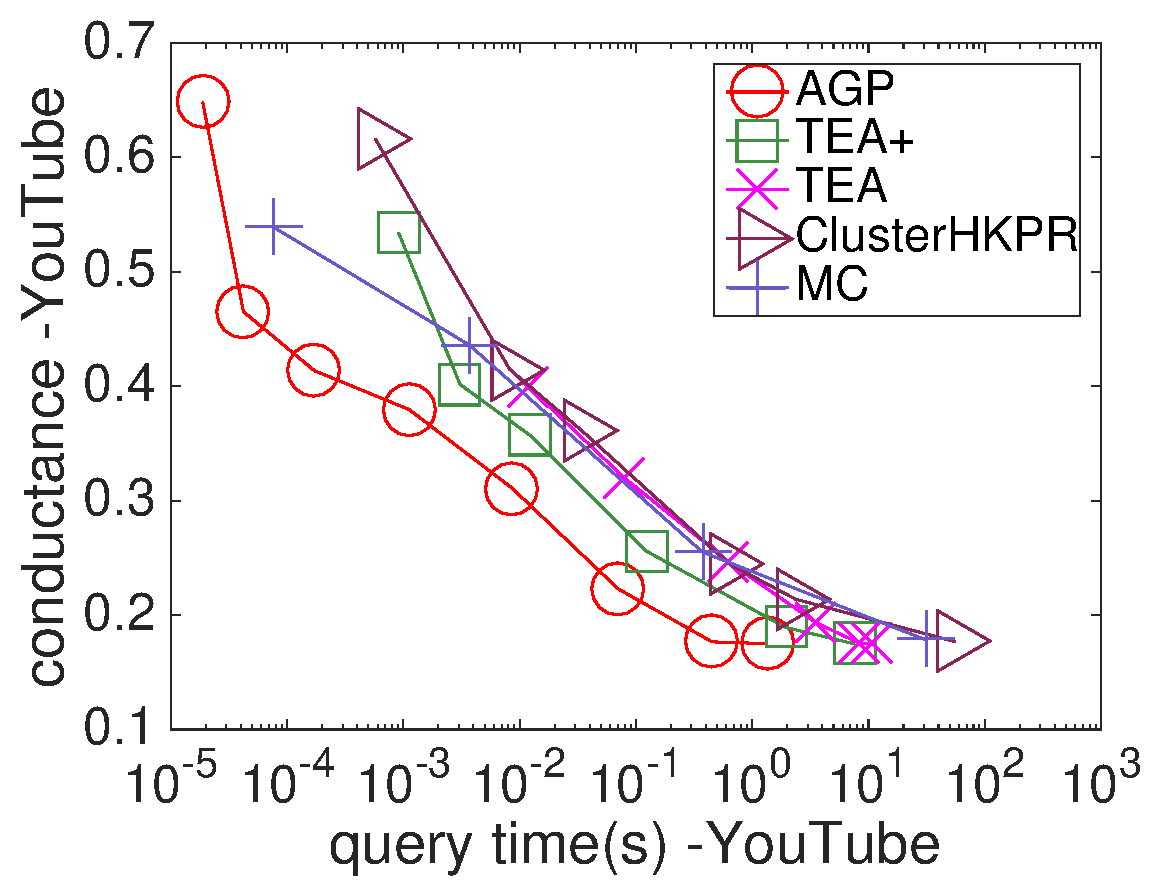
\includegraphics[height=34mm]{./Figs/HKPR-conductance-query-YT.eps} &
% 			%\hspace{-3mm} \includegraphics[height=25mm]{./Figs/HKPR-conductance-query-DB.eps} &
% 			\hspace{-4mm} 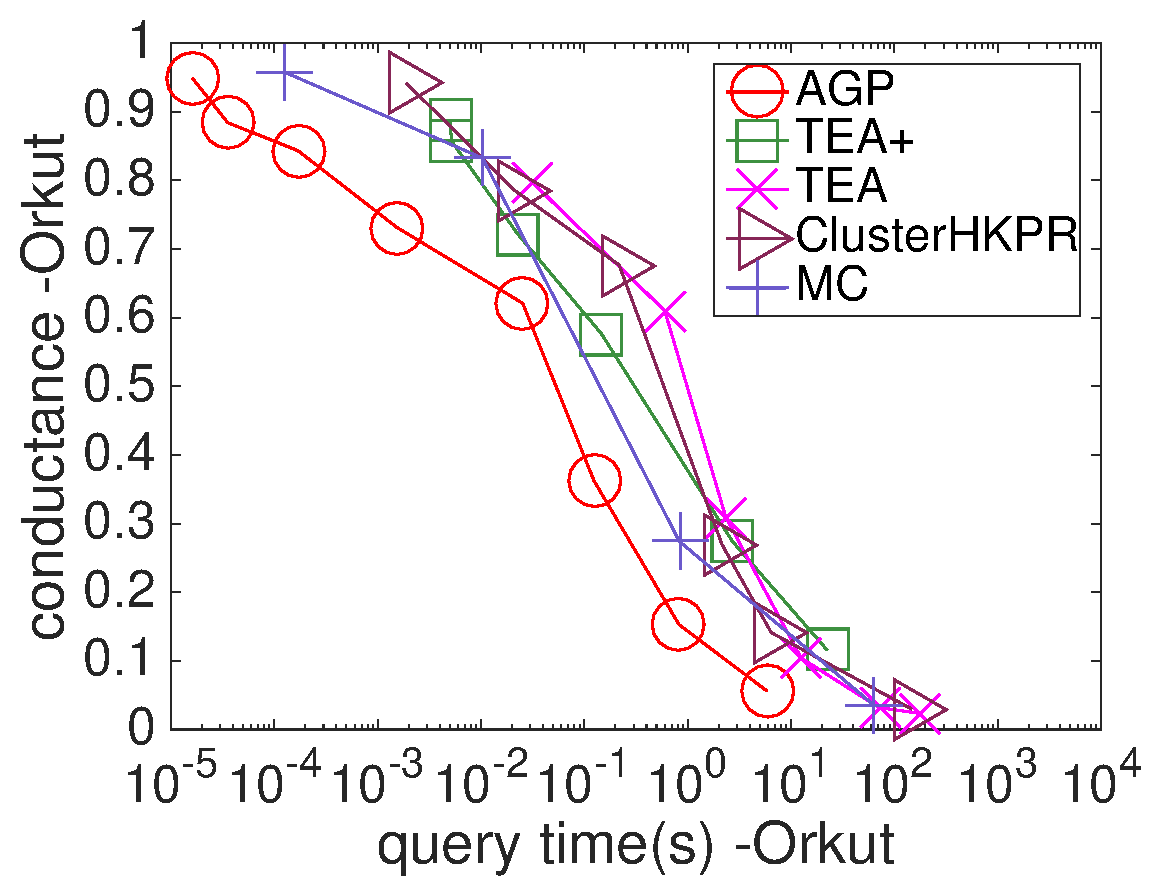
\includegraphics[height=34mm]{./Figs/HKPR-conductance-query-OL.eps} &
% 			\hspace{-4mm} 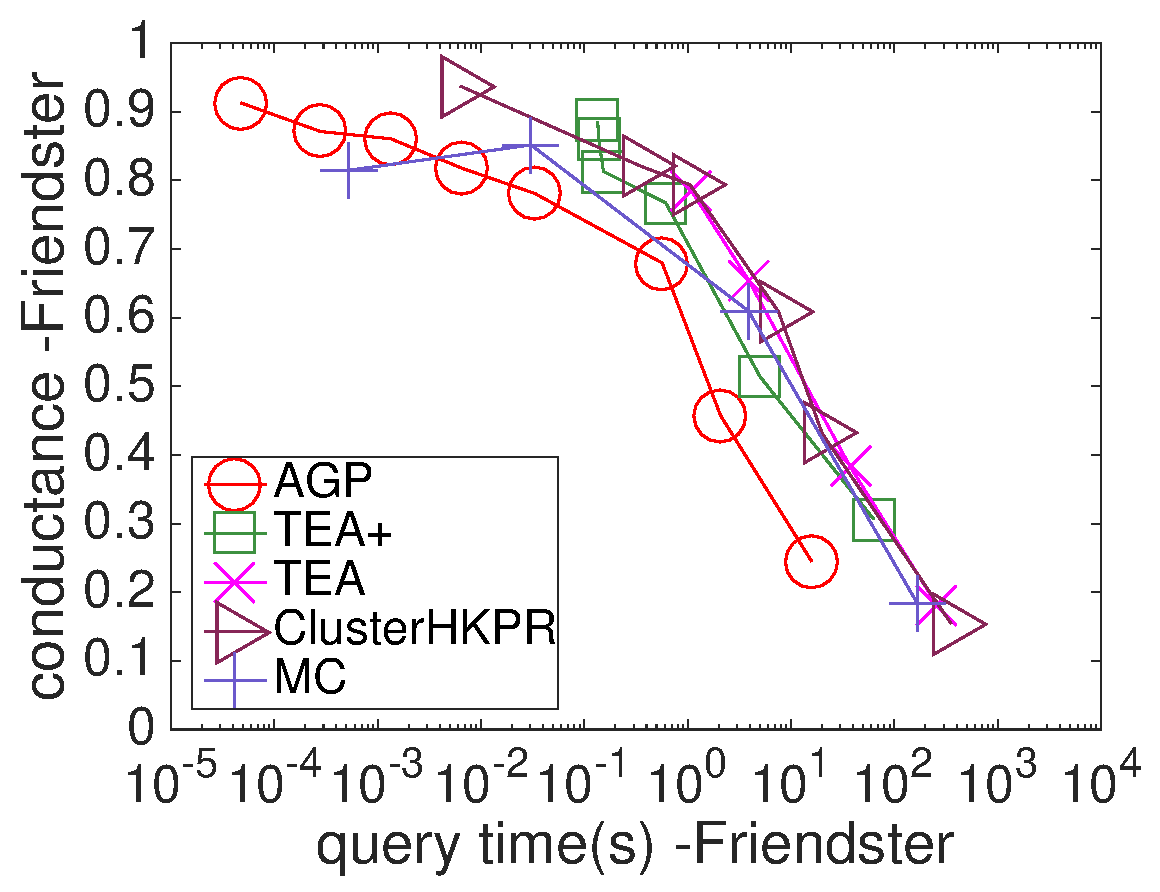
\includegraphics[height=34mm]{./Figs/HKPR-conductance-query-FR.eps} &
% 			%\hspace{-4mm} 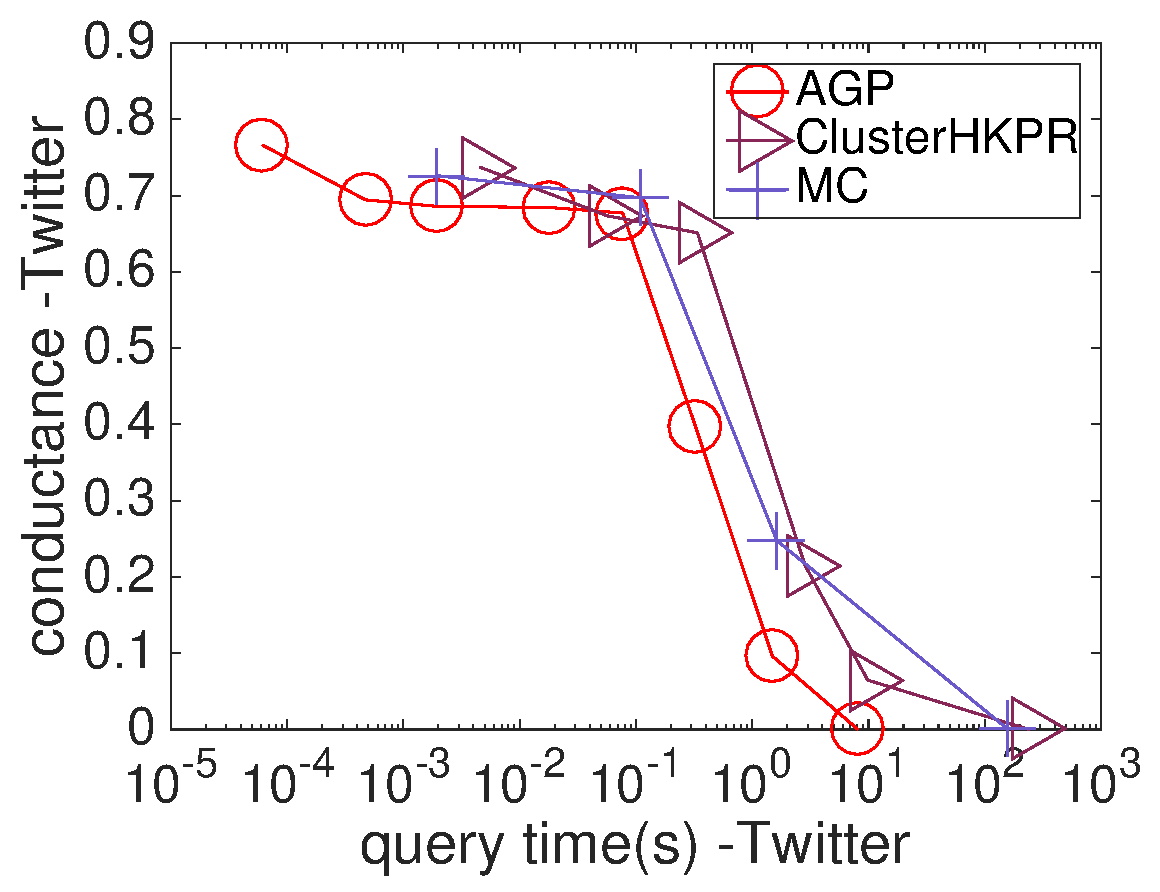
\includegraphics[height=34mm]{./Figs/HKPR-conductance-query-TW.eps} 
% 		\end{tabular}
% 		\vspace{-3mm}
% 		\caption{Tradeoffs between {\em conductance} and query time in local clustering.}
% 		\label{fig:HKPR-conductance-query}
% 		\vspace{-1mm}
% 	\end{small}
% \end{figure*}


\begin{figure*}[t]
	\begin{small}
		\centering
		%\vspace{-5mm}
		%    \begin{footnotesize}
		\begin{tabular}{cccc}
			%\multicolumn{4}{c}{\hspace{-4mm} \includegraphics[height=5mm]{./Figs/legend_large.eps}} \vspace{-1mm} \\
			%\hspace{-3mm} \includegraphics[height=25mm]{./Figs/HKPR-conductance-query-DB.eps} &
			\hspace{-4mm} 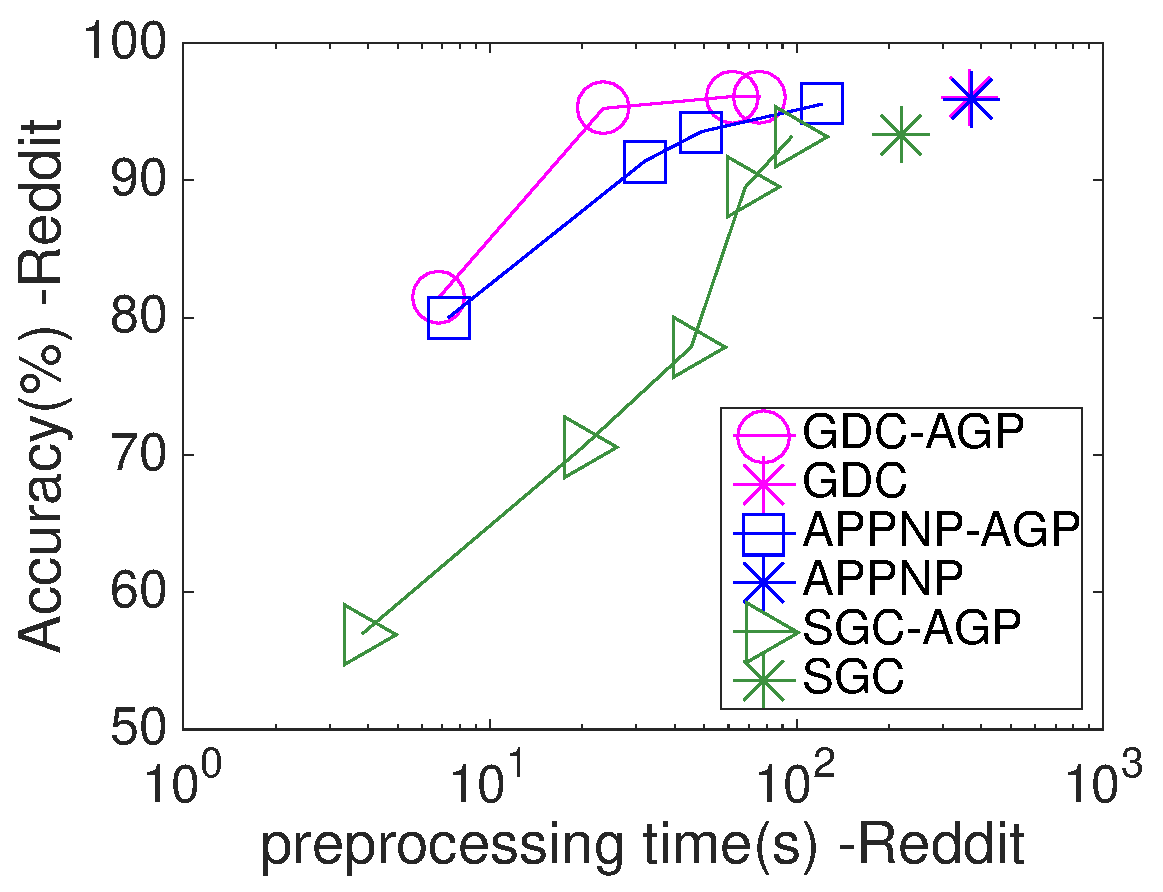
\includegraphics[height=34mm]{./Figs/GNN-accuracy-query-Reddit.eps} &
			\hspace{-4mm} 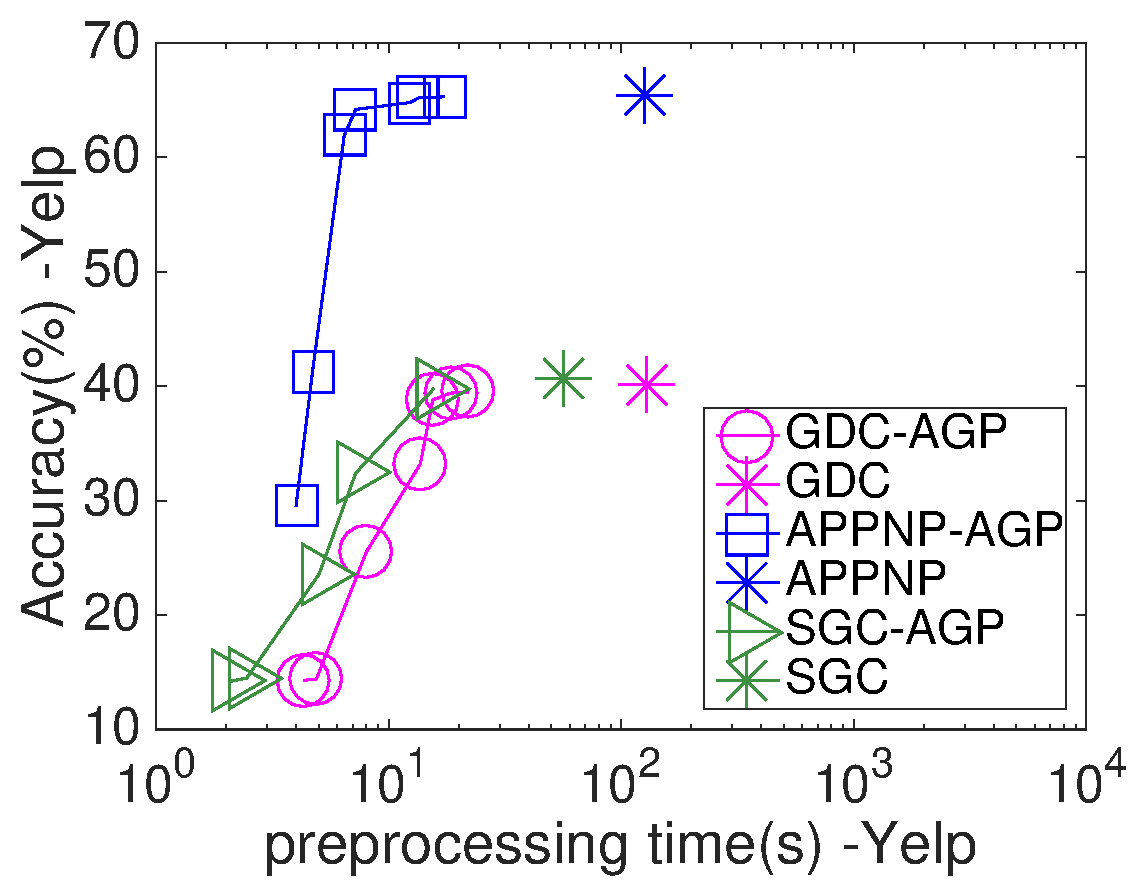
\includegraphics[height=34mm]{./Figs/GNN-accuracy-query-Yelp.eps} &
			\hspace{-2mm} \includegraphics[height=34mm]{./Figs/GNN-accuracy-query-Amazon.eps} &
			\hspace{-4mm} \includegraphics[height=34mm]{./Figs/GNN-accuracy-query-papers100M.eps} 
		\end{tabular}
		\vspace{-5mm}
		\caption{Tradeoffs between {\em Accuracy(\%)} and preprocessing time in node classification (Best viewed in color).}
		\label{fig:GNN-accuracy-query}
		\vspace{-2mm}
	\end{small}
\end{figure*}

\begin{figure}[t]
	\begin{small}
		\centering
		\vspace{-2mm}
		%    \begin{footnotesize}
		\begin{tabular}{cccc}
			%\multicolumn{4}{c}{\hspace{-4mm} \includegraphics[height=5mm]{./Figs/legend_large.eps}} \vspace{-1mm} \\
			%\hspace{-3mm} \includegraphics[height=25mm]{./Figs/HKPR-conductance-query-DB.eps} &
		%	\hspace{-4mm}  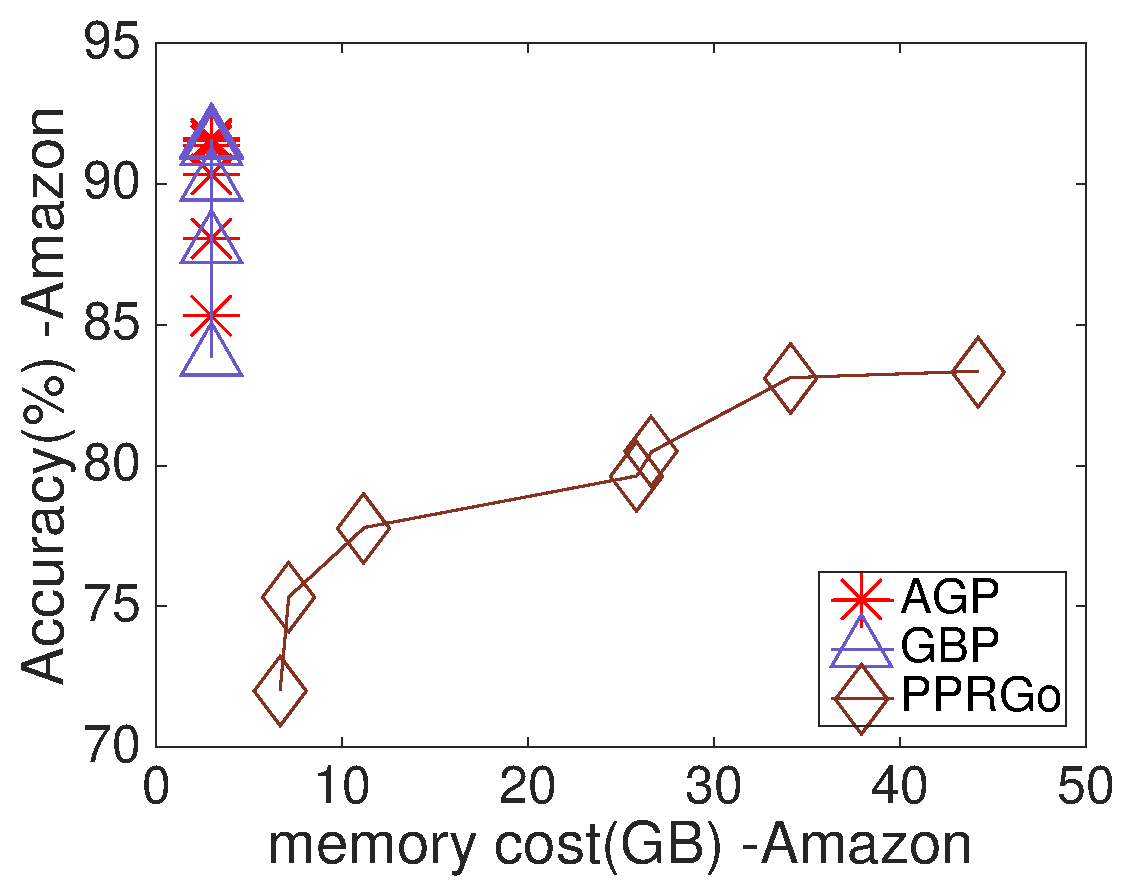
\includegraphics[height=34mm]{./Figs/GNN-accuracy-memory-Amazon.eps} &
			\hspace{-4mm}  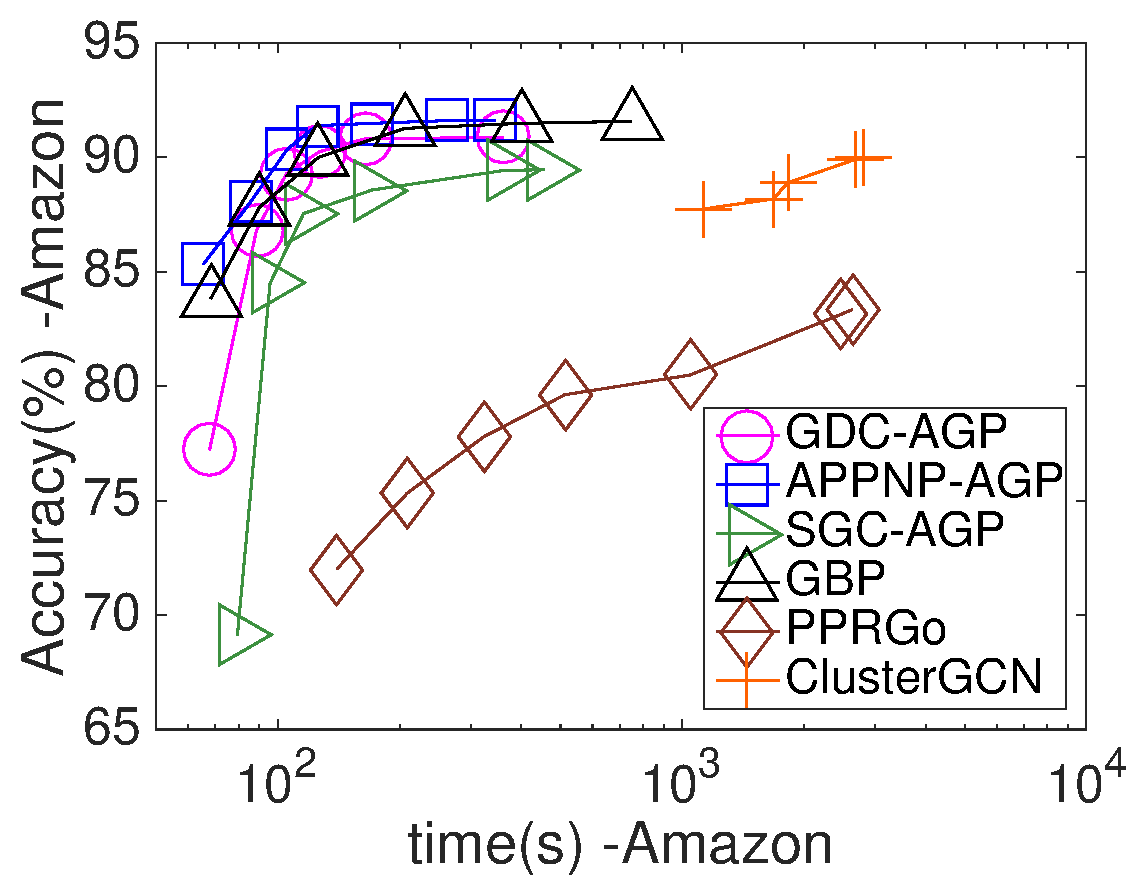
\includegraphics[height=32mm]{./Figs/GNN-accuracy-time-Amazon.eps} &
			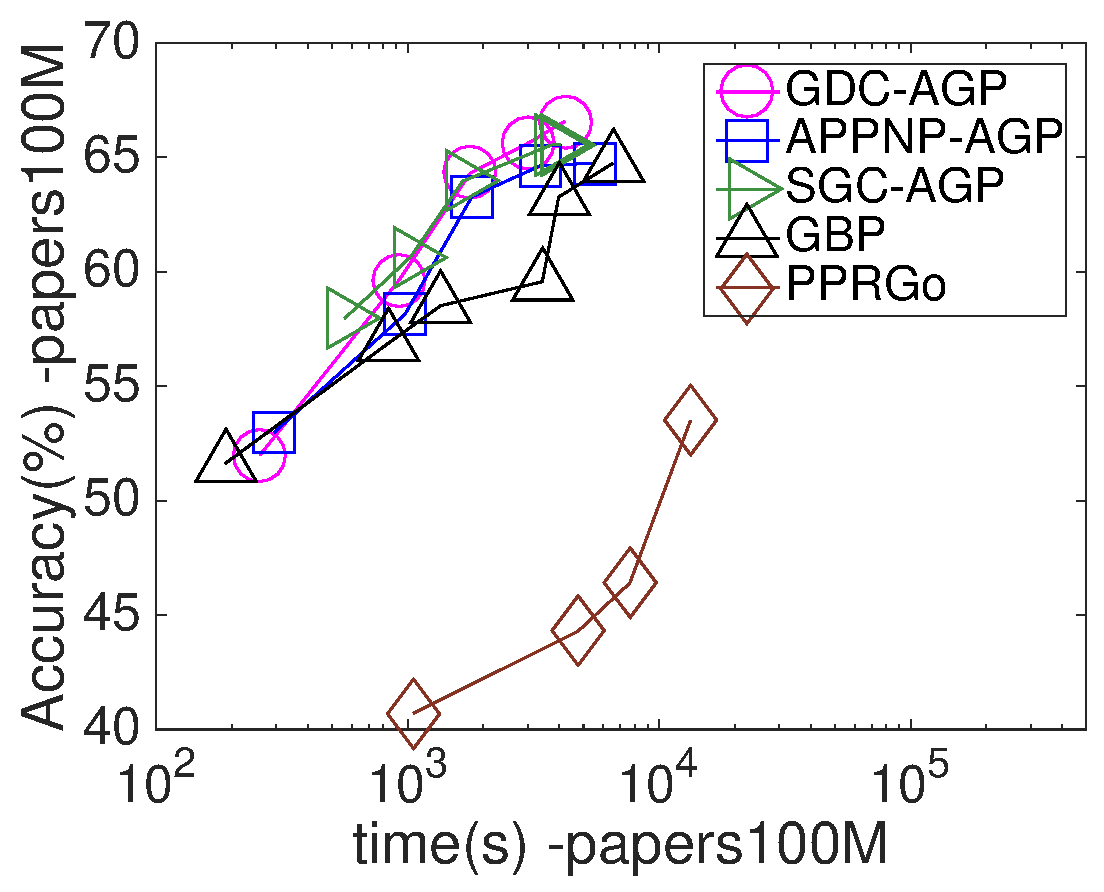
\includegraphics[height=32mm]{./Figs/GNN-accuracy-time-papers100M.eps}
		\end{tabular}
		\vspace{-5mm}
		\caption{Comparison with GBP, PPRGo and ClusterGCN.}
		\label{fig:GBP}
		\vspace{-5mm}
	\end{small}
\end{figure}



\vspace{-2mm}
\subsection{Local clustering with HKPR}\label{subsec:clustering}
In this subsection, we conduct experiments to evaluate the performance of AGP in local clustering problem. We select HKPR among various node proximity measures as it achieves the state-of-the-art result for local clustering~\cite{chung2018computing,kloster2014heat,yang2019TEA}. 
We will evaluate the trade-off curve between the query time and the approximation quality, as well as the trade-off curve between the query time and the clustering quality.
% first evaluate the query efficiency of heat kernel PageRank computed by AGP against other competitors. Then we compare the clustering quality of these methods using the derived HKPR results. Besides, we also exploit the influence of heat kernel parameter $t$ to the query effects of each algorithm. 




% choose one node proximity metric $\vec{\vec{\pi}}_s(t)$ first and approximate corresponding proximity results for each node $t \in V$ on the graph. 
% Next, sort the nodes on the graph in the descending order of $\frac{\vec{\pi}_s(t)}{d_t}$. 
% Finally, conduct the $\bf sweeping$ operation through the sorted nodes to find the subset with minimum conductance as the approximate clustering result. 
% In our experiments, we also obey this structure and apply heat kernel PageRank $\vec{\vec{\pi}}_s=\sum_{i=0}^\infty \frac{e^{-t}t^i}{i!}\cdot \left(\mathbf{A}\mathbf{D}^{-1}\right)^i\cdot \vec{e}_s$ as the node proximity following the state-of-the-art work~\cite{chung2018computing, kloster2014heat, yang2019TEA}. 


%normalize each proximity by
%Then they where heat kernel PageRank(HKPR) is the most commonly used proximity. 

%So in our experiments, we also compute the heat kernel PageRank first for every node on the graph with a given node as the seed. 





\header{\bf Datasets and Environment.} 
%Table~\ref{tbl:datasets} presents the detailed information of the datasets we used for local clustering, which can be obtained from~\cite{snapnets,LWA}. We use three undirected graphs: YouTube, Orkut, and Friendster in our experiments, as most of the local clustering methods can only support undirected graphs. We also use a large directed graph Twitter to demonstrate AGP's effectiveness on directed graphs. All local clustering experiments are conducted on a machine with an Intel(R) Xeon(R) Gold 6126@2.60GHz CPU and 500GB memory.
We use three undirected graphs: YouTube, Orkut, and Friendster in our experiments, as most of the local clustering methods can only support undirected graphs. We also use a large directed graph Twitter to demonstrate AGP's effectiveness on directed graphs. The four datasets can be obtained from~\cite{snapnets,LWA}. We summarize the detailed information of the four datasets in Table~\ref{tbl:datasets}. 



%\header{\bf Methods and Parameters.} 
\header{\bf Methods.} 
We compare AGP with four local clustering methods: TEA~\cite{yang2019TEA} and its optimized version TEA+, ClusterHKPR~\cite{chung2018computing}, and the Monte-Carlo method (MC). We use the results derived by the Basic Propagation Algorithm~\ref{alg:AGP-deter} with $L = 50$ as the ground truths for evaluating the trade-off curves of the approximate algorithms. Detailed descriptions on parameter setting for each method are deferred to appendix due to the space limits. 






\header{\bf Metrics.} 
%We use {\em MaxError} and {\em Precision@k} as our metrics to measure the approximation quality of each method. {\em MaxError} is defined as $MaxError =\max_{v \in V}\left|\frac{\vec{\pi}(v)}{d_v}-\frac{\vec{\epi}(v)}{d_v}\right|$, which measures the maximum error between the true normalized HKPR and the estimated value. Note that we use the basic propagation algorithm~\ref{alg:AGP-deter} with $L=50$ to obtain the ground truths of the normalized HKPR. 
We use {\em MaxError} as our metric to measure the approximation quality of each method. {\em MaxError} is defined as $MaxError =\max_{v \in V}\left|\frac{\vec{\pi}(v)}{d_v}-\frac{\vec{\epi}(v)}{d_v}\right|$, which measures the maximum error between the true normalized HKPR and the estimated value. We refer to $\frac{\vec{\pi}(v)}{d_{v}} $ as the {\em normalized HKPR} value from $s$ to $v$. %Note that we use the basic propagation algorithm~\ref{alg:AGP-deter} with $L=50$ to obtain the ground truths of the normalized HKPR.
On directed graph, $d_v$ is substituted by the out-degree $d_{out}(v)$. 
%We use {\em Precision@k} as our metric to measure the approximation quality of each method. Let $V_k$ denote the set of $k$ nodes with highest normalized HKPR values, and $\hat{V}_k$ denote the estimated top-$k$ node set returned by an approximate mthod. {\em Precision@k} is defined as the percentage of nodes in $\hat{V}_k$ that coincides with the actual top-$k$ results $V_k$. We use {\em Precision@k} to evaluate the accuracy of the relative node order of each method. We use the basic propagation algorithm~\ref{alg:AGP-deter} with $L=50$ to obtain the ground truths of the normalized HKPR. On directed graph, $d_t$ is substituted by the out-degree $d_{out}(v)$. 
 
%We also consider the quality of the cluster. More precisely, after deriving the (approximate )HKPR vector, we sort the nodes in descending order of the normalized HKPR values  and perform a sweeping operation to find the cluster with minimum conductance,  $\Phi(S)=\frac{|cut(S)|}{\min\{vol(S),2m-vol(S)\}}$ to measure the clustering quality, where $vol(S)=\sum_{v \in S}d(v)$, and $cut(S)=\{(u,v)\in E \mid u \in S, v \in V-S \}$. We evaluate the trade-offs between the minimum conductance found by each method and its query time. For each metric, we return the average of 50 randomly selected source nodes.  

%As mentioned in Section~\ref{subsec:cluserting-pre}, we perform local clustering methods with a sweeping algorithm. 
We also consider the quality of the cluster algorithms, which is measured by the {\em conductance}. Given a subset $S  \subseteq V$, the conductance is defined as $\Phi(S)\hspace{-1mm}=\hspace{-1mm}\frac{|cut(S)|}{\min\{vol(S),2m-vol(S)\}}$, where $vol(S)\hspace{-1mm}=\hspace{-1mm}\sum_{v \in S}d(v)$, and $cut(S)\hspace{-1mm}=\hspace{-1mm}\{(u,v)\hspace{-1mm}\in\hspace{-1mm} E \mid u \in S, v \in V-S \}$.
We perform a sweeping algorithm~\cite{Teng2004Nibble,FOCS06_FS,chung2007HKPR,chung2018computing,yang2019TEA} to find a subset $S$ with small conductance. More precisely, after deriving the (approximate) HKPR vector from a source node $s$, we sort the nodes $\{v_1, \ldots, v_n\}$ in descending order of the normalized HKPR values that $\frac{\vec{\pi}(v_1)}{d_{v_1}}\hspace{-1mm}\ge\hspace{-1mm} \frac{\vec{\pi}(v_2)}{d_{v_2}} \hspace{-1mm}\ge \hspace{-1mm}\ldots \hspace{-1mm}\ge \hspace{-1mm}\frac{\vec{\pi}(v_n)}{d_{v_n}}$. %we sort the nodes in descending order of the normalized HKPR values. 
Then, we sweep through $\{v_1, \ldots, v_n\}$ and find the node set with the minimum {\em conductance} among partial sets $S_i\hspace{-1mm} =\hspace{-1mm} \{v_1, \ldots,v_i\}, i\hspace{-1mm}=\hspace{-1mm}1,\ldots,n\hspace{-1mm}-\hspace{-1mm}1 $.

%More precisely, given a node $s$, we compute the HKPR vector $\vec{\pi} = \sum_{i=0}^\infty \frac{e^{-t}t^i}{i!}\cdot \left(\mathbf{A}\mathbf{D}^{-1}\right)^i\cdot \vec{e}_s$ of $s$, and sort the nodes $\{v_1, \ldots, v_n\}$ in descending order of $\frac{\vec{\pi}(v_1)}{d_{v_1}}\ge \frac{\vec{\pi}(v_2)}{d_{v_2}} \ge \ldots \ge \frac{\vec{\pi}(v_n)}{d_{v_n}}$. We refer to $\frac{\vec{\pi}(v)}{d_{v}} $ as the {\em normalized HKPR} value from $s$ to $v$. Then, we sweep through $\{v_1, \ldots, v_n\}$ and find the node set with the minimum conductance among partial sets $S_i = \{v_1, \ldots,v_i\}, i=1,\ldots,n-1 $. 
%After deriving the (approximate )HKPR vector, we perform a sweep algorithm to find the clusters with minimum conductance,  $\Phi(S)=\frac{|cut(S)|}{\min\{vol(S),2m-vol(S)\}}$ to measure the clustering quality, where $vol(S)=\sum_{v \in S}d(v)$, and $cut(S)=\{(u,v)\in E \mid u \in S, v \in V-S \}$. We evaluate the trade-offs between the minimum conductance found by each method and its query time. For each metric, we return the average of 50 randomly selected source nodes. 


 

\header{\bf Experimental Results.}
%Figure~\ref{fig:HKPR-precision-query} plots the trade-off curve between {\em Precision@50} and the query time for each method. We omit TEA and TEA+ on Twitter as they cannot handle directed graphs. We observe that AGP achieves the highest precision among the five approximate algorithms on all four datasets under the same query time. 
Figure~\ref{fig:HKPR-maxerror-query} plots the trade-off curve between the {\em MaxError} and query time. We observe that AGP  achieves the lowest curve among the five algorithms on all four datasets, which means AGP incurs the least error under the same query time. As a generalized algorithm for the graph propagation problem, these results suggest that AGP outperforms the state-of-the-art HKPR algorithms in terms of the approximation quality. 

% $1$ using the least time, which reflects the query efficiency of AGP. Besides, we notice that TEA+ and Monte-Carlo show a better performance than TEA and ClusterHKPR, which concurs with  analysis. In Figure~\ref{fig:HKPR-maxerror-query}, we plot the trade-offs between {\em MaxError} and query time. AGP is also the fastest method to reach the same additive error. Note that AGP can always achieve a $10x$ faster than TEA+ and $20\times-30\times$ faster than Monte-Carlo based methods. 
% Because the algorithm structure of TEA and TEA+ are only for undirected graphs. So we omit the lines of these two methods on the directed graph {\em Twitter}. On {\em Twitter}, AGP still has a better performance than the other Monte-Carlo based methods, which demonstrates the effectiveness of AGP on directed graphs. 

%To evaluate the quality of the clusters found by each method, Figure~\ref{fig:HKPR-conductance-query} shows the trade-off curve between conductance and the query time for each algorithm. We omit Twitter as the conductance metric which is only defined on undirected graphs.  We observe that AGP can achieve the lowest conductance-query time curve among the five approximate methods, which concurs that AGP provides estimators that are closest to the actual normalized HKPR. %ORIGIN!!
To evaluate the quality of the clusters found by each method, Figure~\ref{fig:HKPR-conductance-query} shows the trade-off curve between conductance and the query time on two large undirected graphs Orkut and Friendster. 
We observe that AGP can achieve the lowest conductance-query time curve among the five approximate methods on both of the two datasets, which concurs with the fact that AGP provides estimators that are closest to the actual normalized HKPR. 


%We also observe that as an exact algorithm, the basic propagation algorithm achieves the lowest conductance. 

%Finally,  Figure~\ref{fig:conductance-query-OL} plots the conductance and query time trade-offs on {\em Orkut}, with $t$ varying in $\{5,10,20,40\}$. Recall that $t$ is the average length of the heat kernel random walk. Hence, the query time of each method increases as  $t$ varying from 5 to 40.  We also observe that AGP consistently achieves the lowest conductance with the same amount of query time. Furthermore, as $t$ increases from $5$ to $40$, AGP's query time only increases by $7\times$, while TEA and TEA+ increase by $10\times-100\times$, which demonstrates the scalability of AGP. 

% the same conductance during the least time. Moreover, comparing the query time of each method when $t=5$ and $t=40$, AGP has a $7\times$ time increment, while $11\times$ increment for Monte-Carlo and $10-100\times$ increment for TEA+. This shows the good scalability of AGP. 





% \begin{table}[t]
% %\vspace{-5mm}
% 	\centering
% 	\tblcapup
% 	\caption{Comparison with APPNP, GDC and SGC.}
% 	\vspace{-3mm}
% 	\tblcapdown
% 	\begin{small}
% \begin{tabular}{|c|l|c|r|}
% \hline
% \multicolumn{2}{|c|}{}                  & \multicolumn{1}{l|}{Accuracy} & \multicolumn{1}{l|}{Propagation time(s)} \\ \hline
% \multirow{6}{*}{Amazon} & APPNP  & 91.4  & 454.1  \\ \cline{2-4}
%                 & AGP-APPNP      & 91.3  & 176.3  \\ \cline{2-4} 
%                         & GDC    & 90.8  & 458.2  \\ \cline{2-4}
%                 & AGP-GDC        & 90.8  & 114.7  \\ \cline{2-4}
%                         & SGC    & 89.5  & 271.8  \\ \cline{2-4} 
%                 & AGP-SGC        & 88.9  & 93.6   \\ \hline
                
% \multirow{6}{*}{Yelp} & APPNP    & 65.4  & 127.4  \\ \cline{2-4}
%                 & AGP-APPNP      & 65.4  & 17.3   \\ \cline{2-4}
%                       & GDC      & 39.6  & 129.8  \\ \cline{2-4}
%                 & AGP-GDC        & 39.5  & 18.4   \\ \cline{2-4}
%                       & SGC      & 30.1  & 56.7   \\ \cline{2-4} 
%                 & AGP-SGC        & 29.8  & 15.6   \\ \hline
                
% \multirow{6}{*}{Reddit} & APPNP  & 95.9  & 366.1  \\ \cline{2-4}
%                 & AGP-APPNP      & 95.7  & 87.1   \\ \cline{2-4}
%                         & GDC    & 96.1  & 367.7  \\ \cline{2-4}
%                 & AGP-GDC        & 96.1  & 62.1   \\ \cline{2-4}
%                         & SGC    & 93.5  & 161.4  \\ \cline{2-4} 
%                 & AGP-SGC        & 93.2  & 86.3   \\ \hline
                
% \multirow{6}{*}{Papers100M} 
%                       & APPNP    & 62.3  & 55706.8   \\ \cline{2-4}
%                 & AGP-APPNP       & 62.2  & 9253.7    \\ \cline{2-4}
%                       & GDC      & 64.3  & 51247.1   \\ \cline{2-4}
%                 & AGP-GDC         & 64.1  & 6808.2    \\ \cline{2-4}
%                       & SGC      & 63.4  & 24968.6   \\ \cline{2-4}
%                 & AGP-SGC         & 61.2  & 1437.2    \\ \hline
% \end{tabular}
% \end{small}
% \end{table}


\begin{table}[t]
	\vspace{-3mm}
	\centering
	\tblcapup
	\caption{Datasets for node classification.}
	\vspace{-5mm}
	\tblcapdown
	\begin{small}
		\begin{tabular}{|l|r|r|r|r|r|} %p{1.3in}|}
			\hline
			{\bf Data Set} & {\bf $\boldsymbol{n}$}& {\bf $\boldsymbol{m}$} & {\bf $\boldsymbol{d}$}& {\bf Classes} 	& {\bf Label $\%$}  \\ \hline
    Reddit     & 232,965 &   114,615,892 &602 & 41  & 0.0035           \\
    Yelp        & 716,847     & 6,977,410   & 300 & 100 & 0.7500         \\
    Amazon        & 2,449,029   & 61,859,140  & 100   & 47 & 0.7000      \\
    Papers100M     & 111,059,956 & 1,615,685,872  & 128  &  172 & 0.0109           \\
			\hline
		\end{tabular}
	\end{small}
	\label{tbl:datasets_gnn}
	%\tbldown
	\vspace{-6mm}
\end{table}

\vspace{-2mm}
\subsection{Node classification with GNN}\label{subsec:GNN}
In this section, we evaluate the AGP's ability to scale  existing Graph Neural Network models on large graphs.

\header{\bf Datasets.}
%We use four publicly available graph datasets with different size: a socal network Reddit~\cite{hamilton2017graphSAGE}, a customer interaction network Yelp~\cite{zeng2019graphsaint}, a co-purchasing network Amazon~\cite{chiang2019clusterGCN} and a large citation network Papers100M~\cite{hu2020ogb}. Table~\ref{tbl:datasets_gnn} summarizes the statistics of the datasets. Note that $d$ is the dimension of the node feature, and the label rate is the percentage of labeled nodes in the graph. Following~\cite{zeng2019graphsaint,zou2019layer}, we perform inductive node classification on Yelp, Amazon and Reddit, and semi-supervised transductive node classification on Papers100M. More specifically, for inductive node classification tasks, we train the model on a graph with labeled nodes and predict nodes' labels on a testing graph. For semi-supervised transductive node classification tasks, we train the model with a small subset of labeled nodes and predict other nodes' labels in the same graph. We follow the same training/validation/testing split as previous works in GNN~\cite{zeng2019graphsaint,hu2020ogb}. A detailed discussion on the setting of the experiments can be found in the appendix.
We use four publicly available graph datasets with different size: a socal network Reddit~\cite{hamilton2017graphSAGE}, a customer interaction network Yelp~\cite{zeng2019graphsaint}, a co-purchasing network Amazon~\cite{chiang2019clusterGCN} and a large citation network Papers100M~\cite{hu2020ogb}. Table~\ref{tbl:datasets_gnn} summarizes the statistics of the datasets, where $d$ is the dimension of the node feature, and the label rate is the percentage of labeled nodes in the graph. A detailed discussion on datasets can be found in the appendix. 


% We first evaluate GBP's performance for transductive semi-supervised learning on the three popular citation networks (Cora, Citeseer, and Pubmed). Then we compare GBP with scalable GNN methods three medium to large graphs PPI, Yelp, Amazon in terms of inductive learning ability. Finally, we present the first empirical study of transductive semi-supervised on billion-scale network Friendster. 


%\header{\bf GNN models and detailed setup.} 
\header{\bf GNN models.} 
%%We consider three proximity-based GNN models: APPNP~\cite{Klicpera2018APPNP}, SGC~\cite{wu2019SGC}, and GDC~\cite{klicpera2019GDC}. We augment the three models with the AGP algorithm~\ref{alg:AGP-RQ} to obtain three variants: APPNP-AGP, SGC-AGP and GDC-AGP. Take SGC-AGP as an example. Recall that SGC uses $\mathbf{Z}= \left(\mathbf{D}^{-\frac{1}{2}} \mathbf{A}\mathbf{D}^{-\frac{1}{2}} \right)^L \cdot \X$ to perform feature aggregation, where $\vec{X}$ is the $n\times d$ feature matrix. SGC-AGP treats each column of $\vec{X}$ as a graph signal $\vec{x}$ and perform randomized propagation algorithm (Algorithm~\ref{alg:AGP-RQ}) with predetermined error parameter $\delta$ to obtain the the final representation $\mathbf{Z}$. To achieve high parallelism, we perform propagation for multiple columns of $\mathbf{X}$ in parallel. 
We first consider three proximity-based GNN models: APPNP~\cite{Klicpera2018APPNP},SGC~\cite{wu2019SGC}, and GDC~\cite{klicpera2019GDC}. We augment the three models with the AGP Algorithm~\ref{alg:AGP-RQ} to obtain three variants: APPNP-AGP, SGC-AGP and GDC-AGP. Besides, we also compare AGP with three scalable methods: PPRGo~\cite{bojchevski2020scaling}, GBP~\cite{chen2020GBP}, and ClusterGCN~\cite{chiang2019clusterGCN}. 


%We first consider three proximity-based GNN models: APPNP~\cite{Klicpera2018APPNP},SGC~\cite{wu2019SGC}, and GDC~\cite{klicpera2019GDC}. We augment the three models with the AGP Algorithm~\ref{alg:AGP-RQ} to obtain three variants: APPNP-AGP, SGC-AGP and GDC-AGP. Take SGC-AGP as an example. Recall that SGC uses $\mathbf{Z}=\left(\mathbf{D}^{-\frac{1}{2}} \mathbf{A}\mathbf{D}^{-\frac{1}{2}} \right)^L \hspace{-1mm}\cdot \X$ to perform feature aggregation, where $\X$ is the $n\times d$ feature matrix. SGC-AGP treats each column of $\X$ as a graph signal $\bm{x}$ and perform randomized propagation algorithm (Algorithm~\ref{alg:AGP-RQ}) with predetermined error parameter $\delta$ to obtain the the final representation $\mathbf{Z}$. To achieve high parallelism, we perform propagation for multiple columns of $\mathbf{X}$ in parallel. Since APPNP and GDC's original implementation cannot scale on billion-edge graph Papers100M, we implement APPNP and GDC in the AGP framework. In particular, we set $\varepsilon = 0$ in Algorithm~\ref{alg:AGP-RQ} to obtain the exact propagation matrix $\mathbf{Z}$, in which case the approximate models APPNP-AGP and GDC-AGP essentially become the exact models APPNP and GDC. We set $L\hspace{-1mm}=\hspace{-1mm}20$ for GDC-AGP and APPNP-AGP, and $L\hspace{-1mm}=\hspace{-1mm}10$ for SGC-AGP. Note that SGC suffers from the over-smoothing problem when the number of layers $L$ is large~\cite{wu2019SGC}. We vary the parameter $\varepsilon$ to obtain a trade-off curve between the classification accuracy and the computation time. 


%%Finally, we also include PPRGo~\cite{bojchevski2020scaling}, the state-of-the-art method that improves the scalability of APPNP. PPRGo has three main parameters: the number of non-zero PPR values for each training node $k$, the number of hops $L$, and the residue threshold $r_{max}$. We vary the three parameters $(k, L, r_{max})$ to form a trade-off curve between the classification accuracy and the computation time. 

%Besides, we also compare AGP with three scalable methods: PPRGo~\cite{bojchevski2020scaling}, GBP~\cite{chen2020GBP}, and ClusterGCN~\cite{chiang2019clusterGCN}. Recall that PPRGo is an improvement work of APPNP. It has three main parameters: the number of non-zero PPR values for each training node $k$, the number of hops $L$, and the residue threshold $r_{max}$. %We vary the three parameters $(k, L, r_{max})$ to form a trade-off curve between the classification accuracy and the computation time. We vary the three parameters $(k,L,r_{max})$ from $(32,2,0.1)$ to $(64,10,10^{-5})$. GBP decouples the feature propagation and prediction to achieve high scalability. In the propagation process, GBP has two parameters: the propagation threshold $r_{max}$ and the level $L$. We vary $r_{max}$ from $10^{-4}$ to $10^{-10}$, and set $L=4$. ClusterGCN uses graph sampling method to partition graphs into small parts, and performs the feature propagation on one randomly picked sub-graph in each mini-batch. We vary the partition numbers from $10^4$ to $10^5$, and the propagation layers from $2$ to $4$. For AGP, we vary $\delta$ from $10^{-5}$ to $10^{-10}$, and tune $a,b,w_i$ for the best performance. %Detailed parameter settings can be founded in the appendix. 


%%For each method, we apply a neural network with two hidden layers, trained with mini-batch SGD. The batch size is set to be $10000$ for faster training time and better generalization ability. We employ initial residual connection~\cite{He2016ResNet} across the hidden layers to facilitate training. We use the trained model to predict each testing node's labels and take the mean accuracy after five runs. For each method, we divide the computation time into two parts: the {\em propagation time} for computing $\mathbf{Z}$, and the {\em training time} for performing mini-batch SGD on the 2-layer neural network on $\mathbf{Z}$ until convergence.


%For each method, we apply a neural network with 4 hidden layers, trained with mini-batch SGD. %The batch size is set to be $10000$ for faster training time and better generalization ability. We employ initial residual connection~\cite{He2016ResNet} across the hidden layers to facilitate training. We use the trained model to predict each testing node's labels and take the mean accuracy after five runs. For GDC, APPNP, and SGC, we divide the computation time into two parts: the {\em preprocessing time} for computing $\mathbf{Z}$, and the {\em training time} for performing mini-batch SGD on $\mathbf{Z}$ until convergence. 



\header{\bf Experimental results.} Figure~\ref{fig:GNN-accuracy-query} shows the trade-off between the preprocessing time and classification accuracy for SGC, APPNP, GDC and the corresponding AGP models. For each dataset, the three snowflakes represent the exact methods SGC, APPNP, and GDC, which can be distinguished by colors.
We observe that compared to the exact models, the approximate models generally achieve a $10\times$ speedup in preprocessing time without sacrificing the classification accuracy. For example, on the billion-edge graph Papers100M,  SGC-AGP achieves an accuracy of $62\%$ in less than $2,000$ seconds, while the exact model SGC needs over $20,000$ seconds to finish. %We also observe that APPNP-AGP achieves a higher trade-off curve than PPRGo does, which means AGP is more efficient than PPRGo in terms of scaling PPR-based GNN on large graphs. %To eliminate the effect of parallelism, we also present each method's clock time in the appendix of the technical report~\cite{TechnicalReport} . The results concur with what we found in Figure~\ref{fig:GNN-accuracy-query}. 

Figure~\ref{fig:GBP} shows the performances of AGP compared with PPRGo, GBP, and ClusterGCN on Amazon and Papers100M, the largest publicly available graphs for inductive and transductive node classification tasks, respectively.
We present the trade-off plots between the total computation time and classification accuracy for each model. We report the total running time (i.e., preprocessing time plus training time). 

We omit ClusterGCN on Papers100M as it runs out of 512GB memory on this graph. We observe that AGP significantly outperforms PPRGo and ClusterGCN on both Amazon and Papers100M in terms of both accuracy and running time. Furthermore, given the same running time, AGP achieves a higher accuracy than GBP does on Papers100M. We attribute this quality to the randomization introduced in AGP.





%Figure~\ref{fig:GNN-accuracy-memory} shows the memory overhead of each approximate method. Recall that the AGP algorithm~\ref{alg:AGP-RQ} only maintains two $n$ dimension vectors: the residue vector $\vec{r}$ and the reserve vector $\vec{q}$. Consequently, AGP only takes a fixed memory, which can be ignored compared to the graph's size and the feature matrix.  Such property is ideal for scaling GNN models on massive graphs. On the other hand, PPRGo requires a large memory size to store the intermediate local push results from each training node.






 % Besides, it set the maximum length of walk as $K=t\cdot \frac{\log{1/\delta}}{\log{\log{1/\delta}}}$. When the poisson random number $k$ is large than $K$, it truncate the walk at its $K_{th}$ step. For ClusterHKPR, 
% To obtain a tradeoff curve between the approximation quality and query time, we vary $\delta$ from $0.5$ to $0.0001$ in our experiments. 
%and generate $\frac{16\log{n}}{\delta^2 }$ walks from the seed, instead of $$. 
%evaluates the performance of AGP against state-of-the-art methods.


%%% Local Variables:
%%% mode: latex
%%% TeX-master: "paper"
%%% End:
